\documentclass[a4paper, 11pt]{article}
\usepackage[polish]{babel}
\usepackage[T1]{fontenc}
\usepackage{hyperref}
\usepackage{array}
\usepackage{amssymb}
\usepackage{amsmath}
\usepackage{changepage}
\usepackage{multicol}
\usepackage[margin=1in]{geometry}
\hypersetup{
    colorlinks,
    citecolor=black,
    filecolor=black,
    linkcolor=black,
    urlcolor=black
}
\usepackage{graphicx}

\usepackage{tikz}
\usetikzlibrary{fit,arrows,matrix,positioning, calc, shapes.gates.logic.IEC, shapes.gates.logic.US}
\usetikzlibrary {arrows.meta}
\tikzstyle{branch}=[fill,shape=circle,minimum size=3pt,inner sep=0pt]


\title{%
        \vspace{-1cm}
       \large Sprawozdanie Laboratorium Fizyka dla informatyków \\
       \huge Badanie Transformatora.}

\author{Stanisław Fiedler 160250}
\date{LAB 2, 12 listopada 2024}

\begin{document}
\begin{table}
	\begin{adjustwidth}{-0.25\textwidth}{-0.25\textwidth}
		\begin{center}
			\begin{tabular}{|l|l|l|l|l|}
				\hline
				Nr Ćwiczenia 202                                             & Data wykonania 26.11.2024                 & Wydział WIiT & Semestr 3 & Grupa LAB L1 \\
				\hline
				\multicolumn{2}{|l|}{ Prowadzący: mgr inż. Taras Zhezhera  } & \multicolumn{2}{|l|}{ Stanisław Fiedler } & Ocena:                                  \\
				\hline
			\end{tabular}
		\end{center}
	\end{adjustwidth}
\end{table}

\maketitle
\tableofcontents

\section{Wstęp teoretyczny}\label{sec:wstep} % (fold)
\subsection{Transformator}
Transformator jest urządzeniem służącym on do zamiany napięcia i natężenia prądu przemiennego na inne
napięcie i natężenie prądu bez zmiany częstotliwości prądu.
Transformator składa się z ferromagnetycznego rdzenia i co najmniej dwóch uzwojeń (cewek)
nawiniętych na niego.

Zasada działania transformatora opiera się na zjawisku indukcji elektromagnetycznej. Rozróżniamy trzy
podstawowe stany pracy transformatora: stan jałowy, stan zwarcia oraz stan obciążenia.

\pagebreak
\subsection{Stan jałowy}
W stanie jałowym uzwojenie pierwotne podłączone jest do źródła prądu przemiennego, a uzwojenie wtórne jest rozwarte.
Prąd przemienny w uzwojeniu pierwotnym indukuje w rdzeniu przemienny strumień magnetyczny,
który powoduje powstanie sił elektromotorycznych w uzwojeniach.
Dzięki pomijanie małym rezystancją uzwojeń możemy przyjąć, że chwilowe spadki napięć są równe
indukowanym w nich siłom elektromotorycznym. A zastępując chwilowe spadki napięć na uzwojeniach napięciami skutecznymi otrzymujemy:
\begin{equation}
	\frac{U_1}{U_2} = \frac{n_1}{n_2} = K
\end{equation}
Gdzie $K$ nazywamy przekładnią transformatora.

\subsection{Stan zwarcia}
W stanie zwarcia uzwojenie pierwotne jest połączone ze źródłem prądu przemiennego, a uzwojenie wtórne jest zwarte.
W uzwojeniu wtórnym pod wpływem indukcji pojawia się prąd przemienny.
Korzystając z zasady zachowania energii, stwierdzić,
że moc przekazywana przez źródło do uzwojenia pierwotnego jest równa mocy przekazywanej do
obwodu wtórnego.
Dzięki temu otrzymujemy:
\begin{equation}
	\frac{I_1}{I_2} = \frac{n_2}{n_1} = \frac{1}{K}
\end{equation}


\subsection{Stan obciążenia}
W stanie zwarcia uzwojenie pierwotne jest połączone ze źródłem prądu przemiennego, a uzwojenie wtórne jest połączony z odbiornikiem o skończonej rezystancji.
W tej sytuacji
stosunek napięć w uzwojeniu pierwotnym i wtórnym nie jest równy przekładni transformatora.
Badając więc napięcie na uzwojeniu wtórnym, obserwujemy jego spadek
wraz ze wzrostem natężenia prądu płynącego w tym uzwojeniu.

\subsection{Sprawność}
Sprawność transformatora jest stosunkiem mocy oddanej $P_2$ do mody pobranej ze źródła.
\begin{equation}
	\eta = \frac{P_2}{P_1} \cdot 100\%
\end{equation}
Przybliżając kąty przesunięcia fazowego pomiędzy napięciem i natężeniem prądu w obwodach
pierwotnym i wtórnym otrzymujemy wzór:
\begin{equation}
	\eta = \frac{U_2I_2}{U_1I_1} \cdot 100\%
\end{equation}

% section wstep (end)

\section{Wyniki pomiarów}\label{sec:wyniki_pomiarow} % (fold)
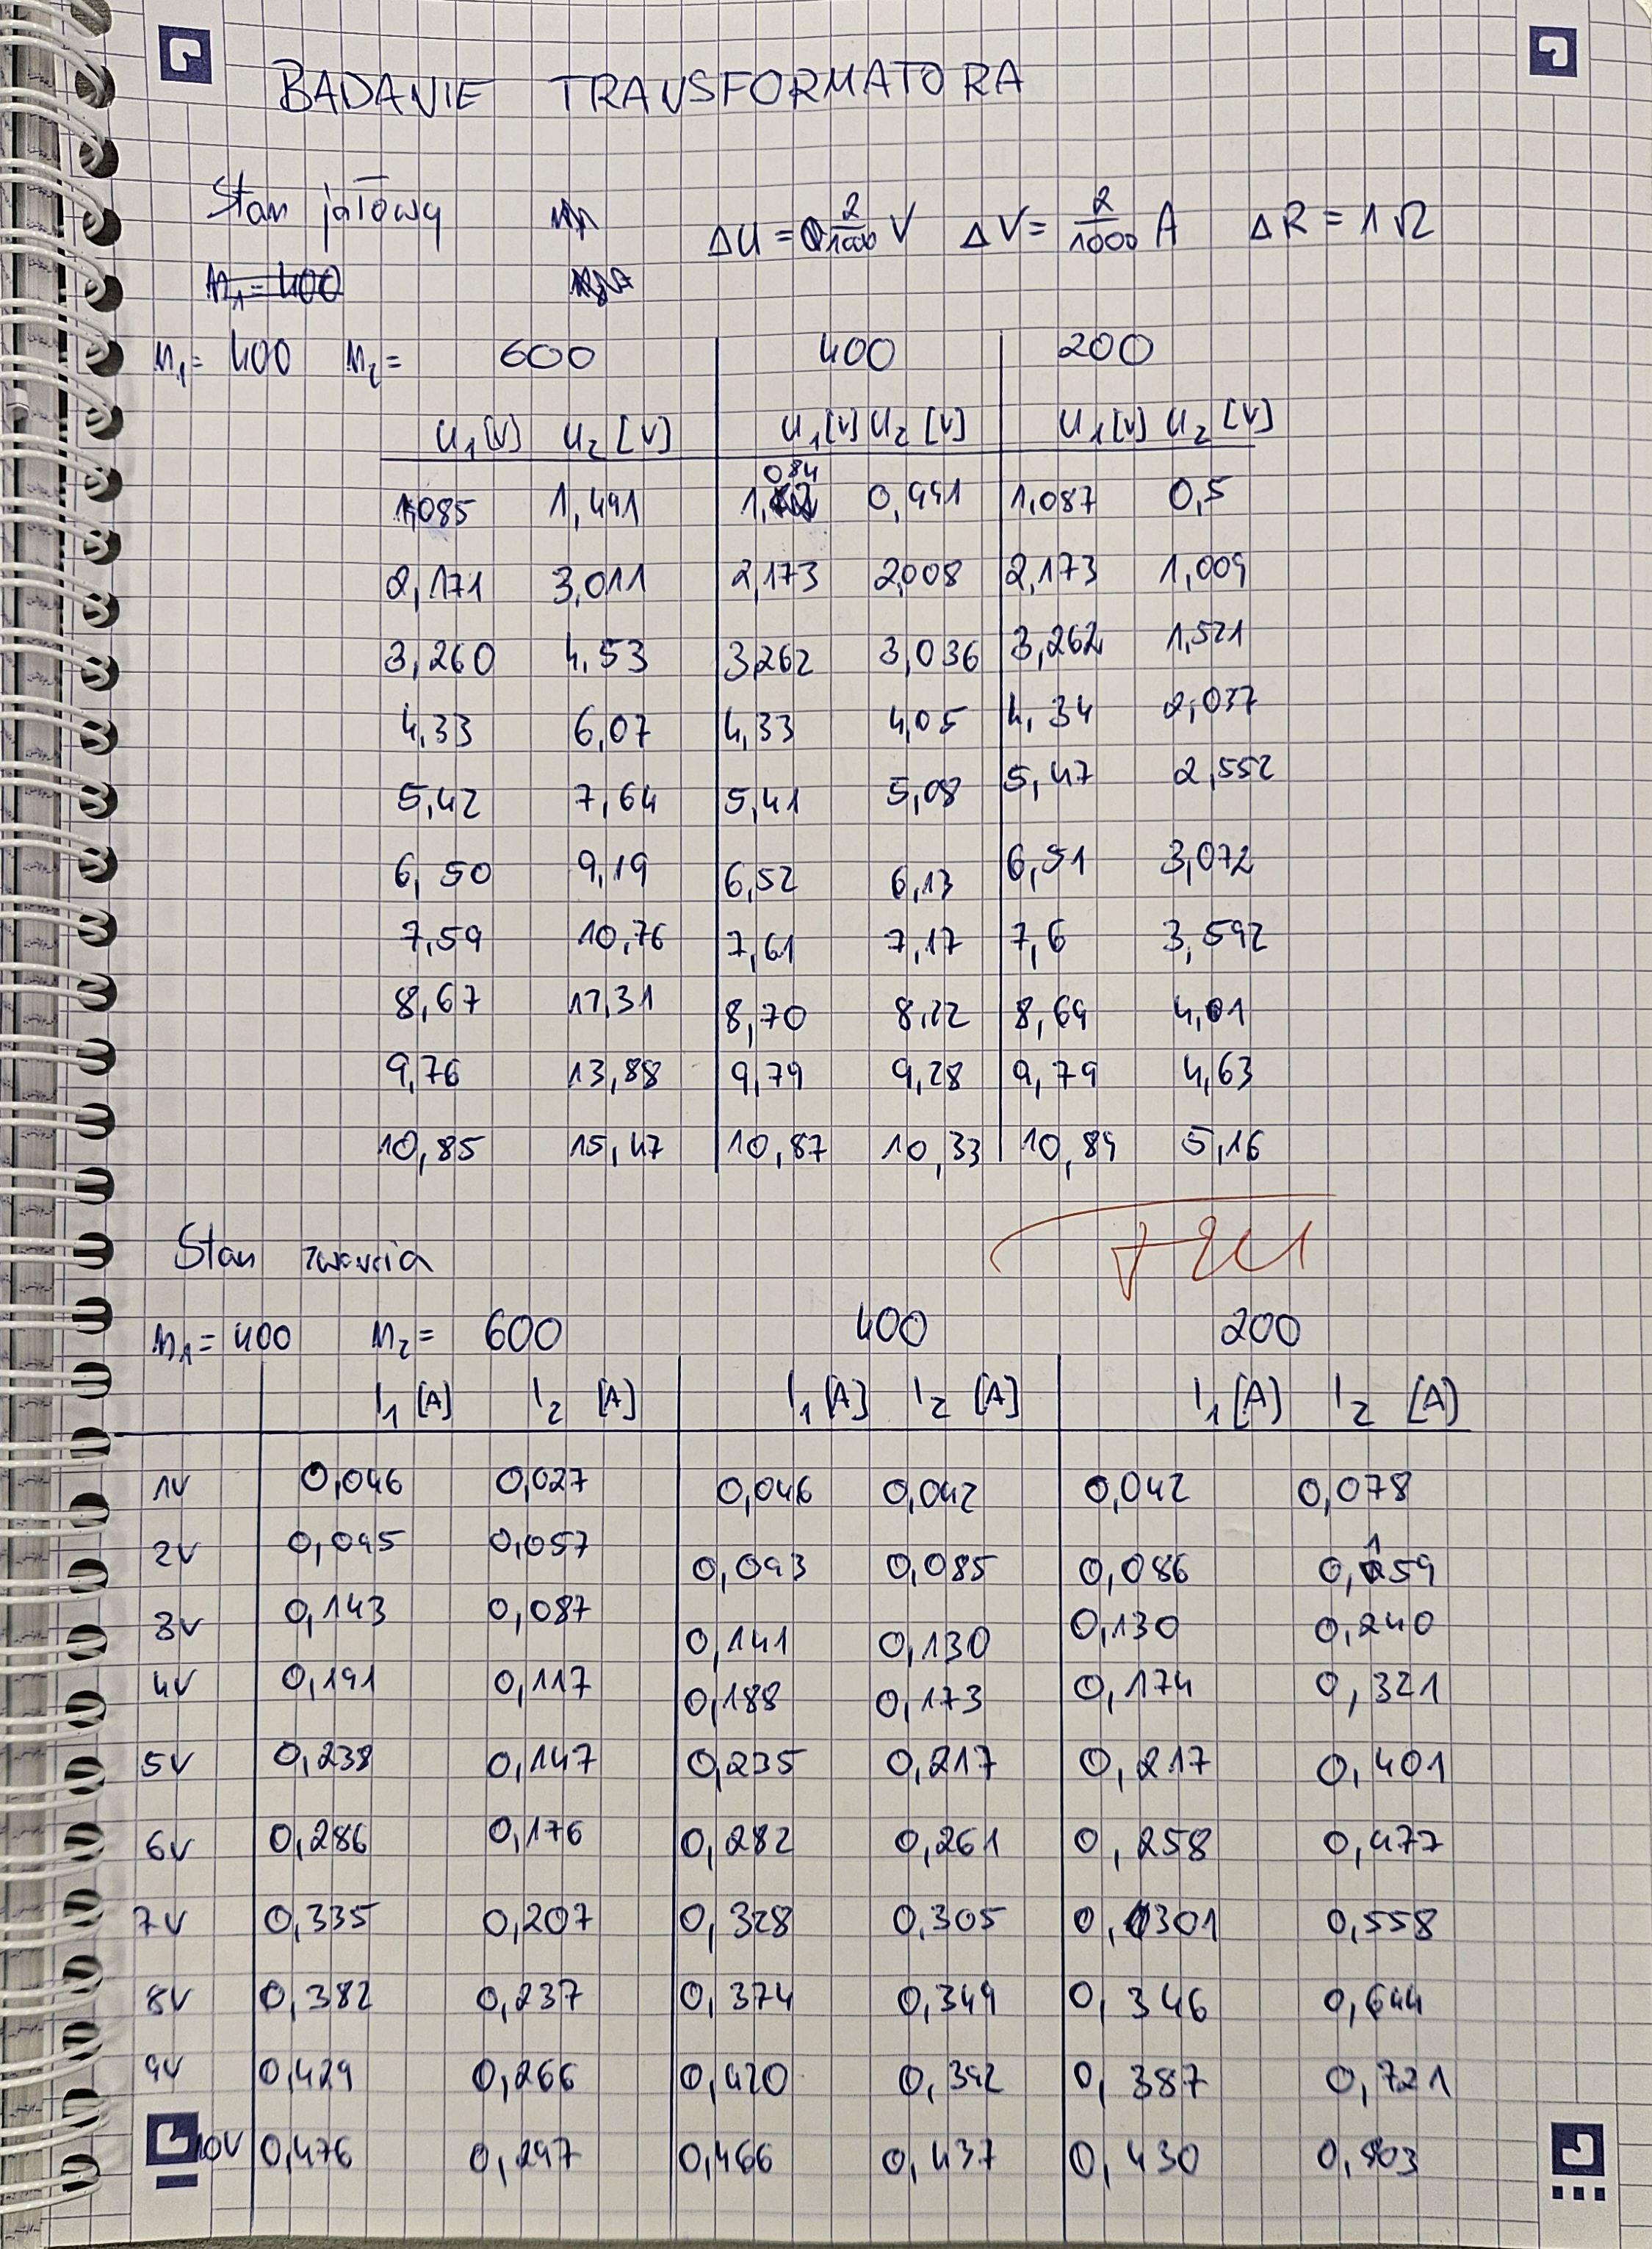
\includegraphics[scale=0.2]{images/img1.jpg}

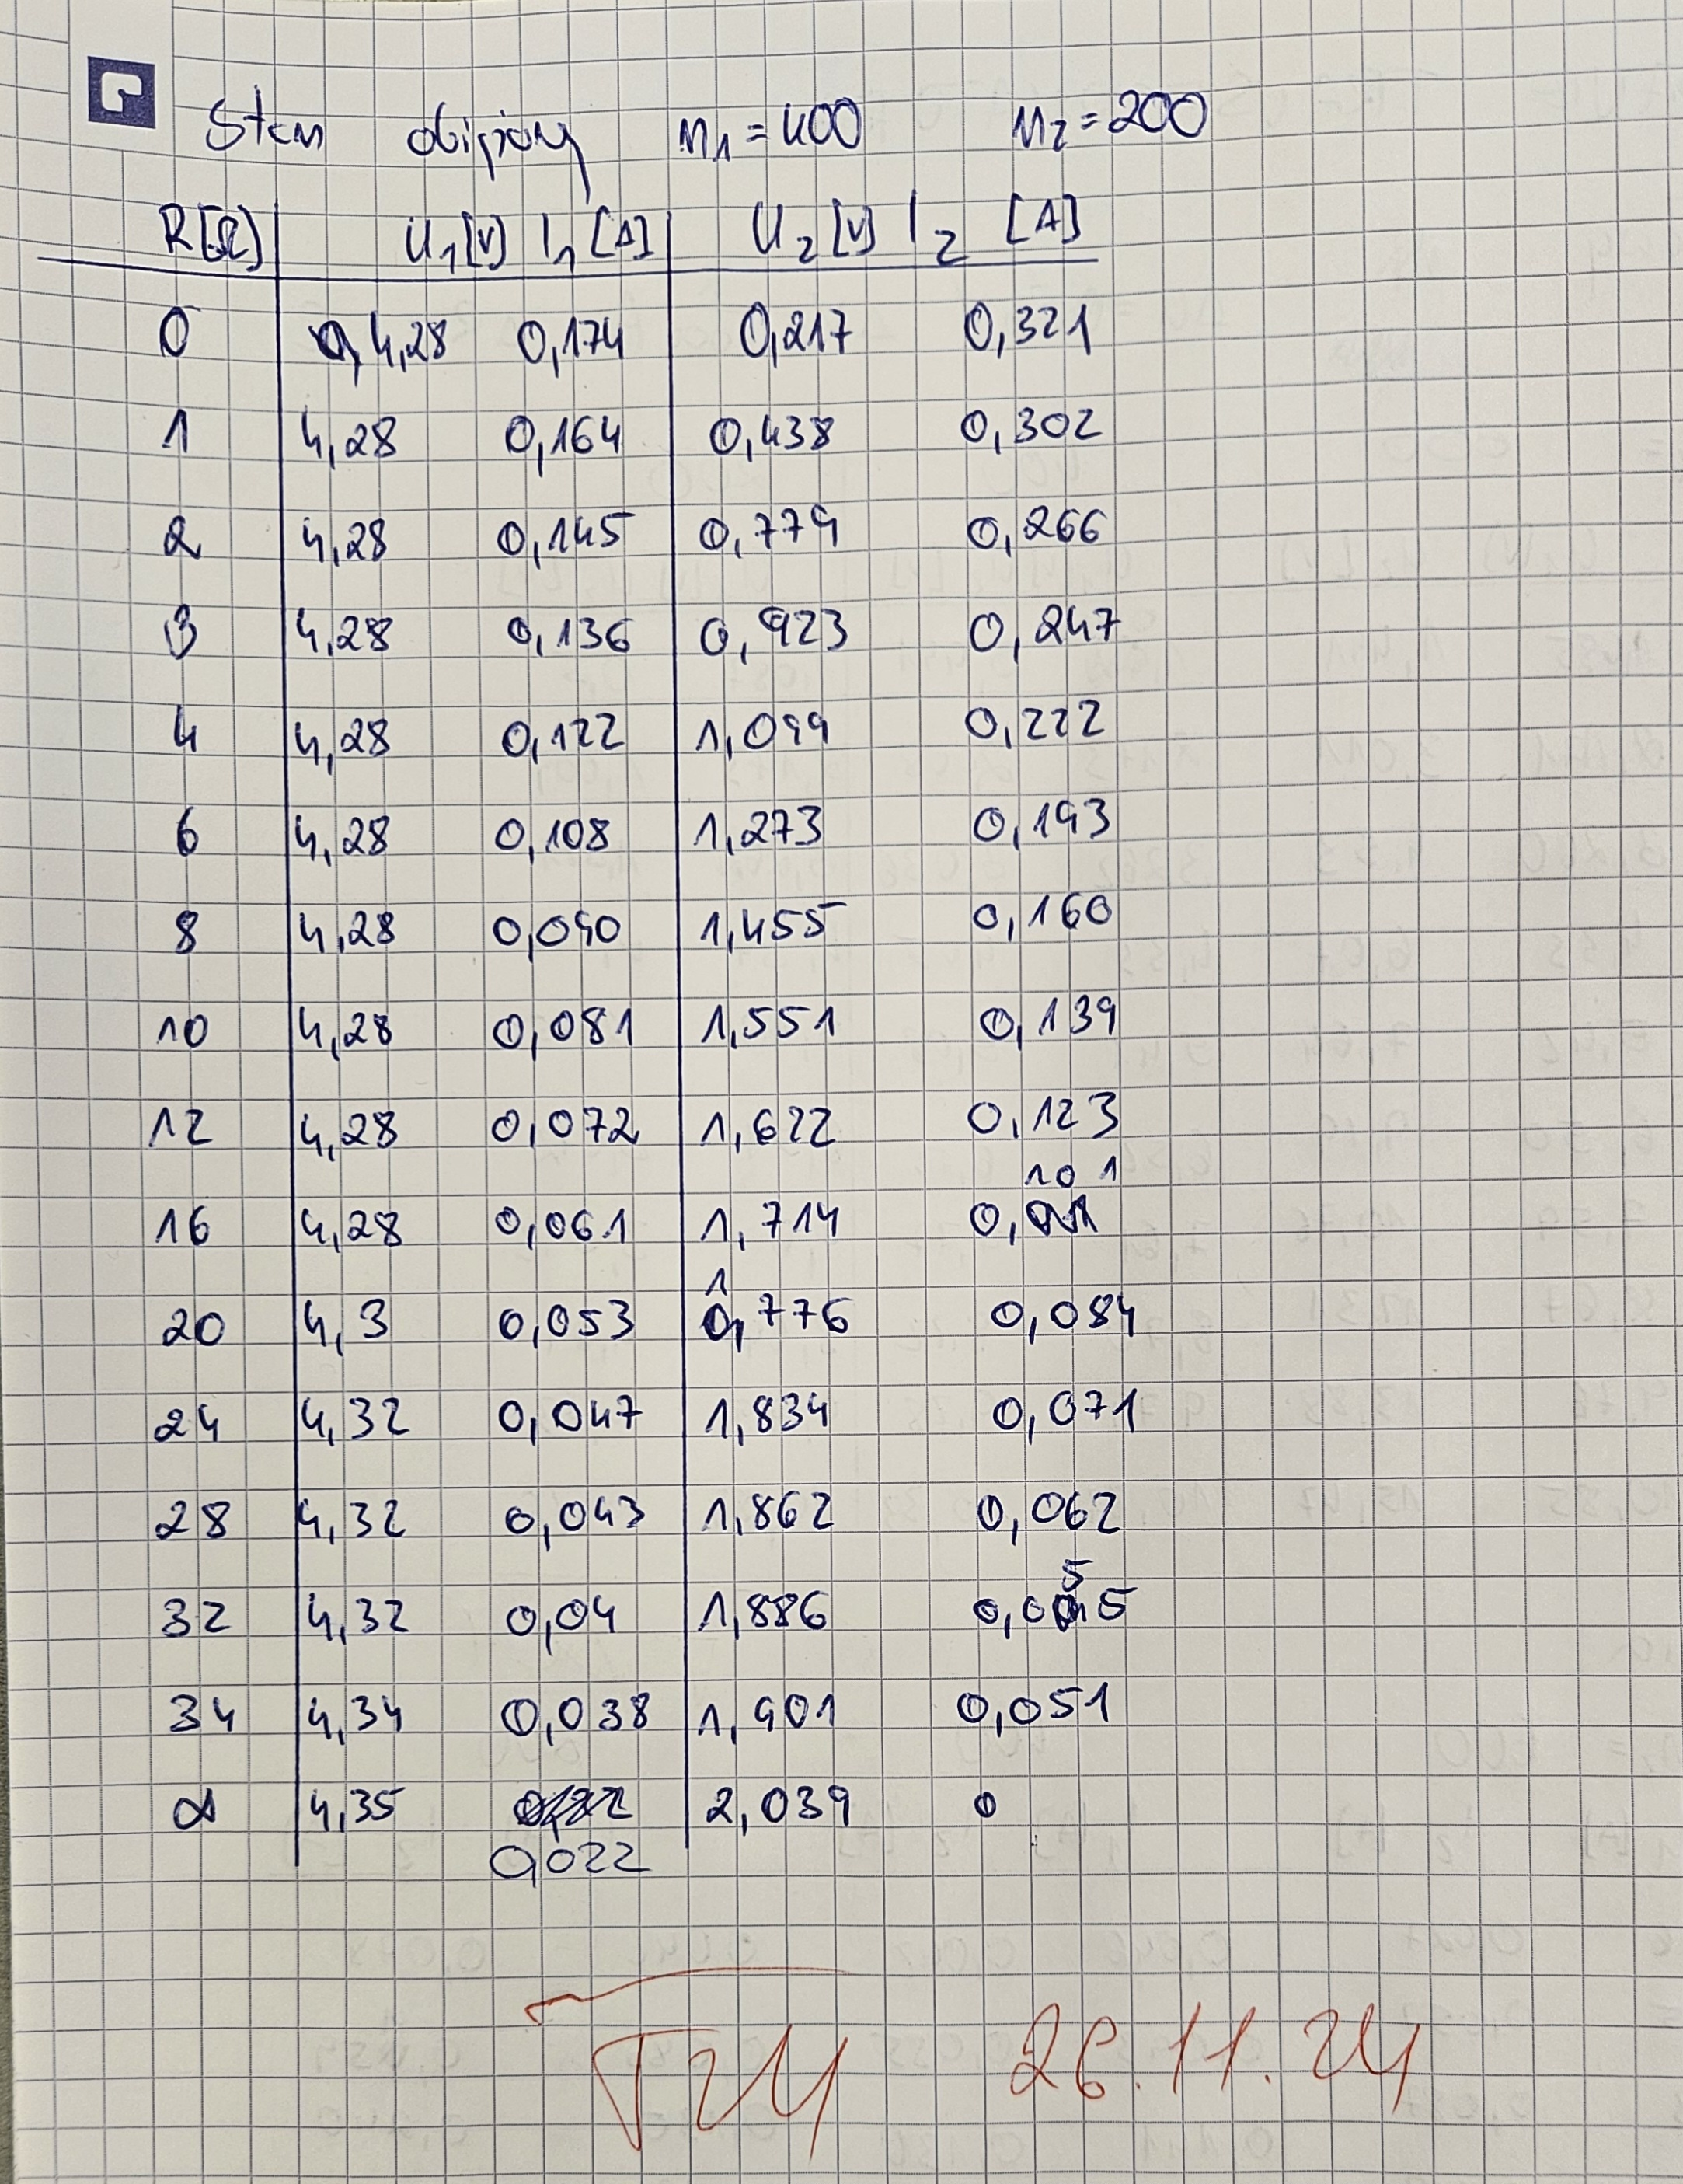
\includegraphics[scale=0.2]{images/img2.jpg}
\pagebreak
% subsection Zdjecie wynikow pomiarow (end)

\section{Opracowanie wyników}\label{sec:opracowanie_wynikow} % (fold)

\subsection{Przekładnia transformatora}\label{sub:przekladnia} % (fold)
\begin{center}
	\large Zależności napięcia wtórnego od napięcia pierwotnego
	$U_2 = f(U_1)$
	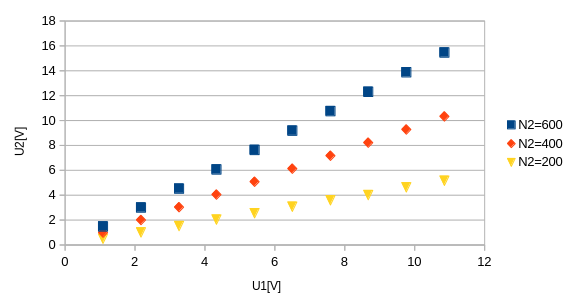
\includegraphics[scale=0.8]{images/1.png}
\end{center}

\subsubsection{Obliczenia}

Przekładnia transformatora zostanie obliczona na podstawie wzoru:

\[
	\frac{U_1}{U_2} = \frac{n_1}{n_2} = K
\]

\begin{multicols}{3}
	$n_1 = 400 \quad n_2 = 600$
	\begin{tabular}{l|l|l}
		\hline
		$V_1 [V]$ & $V_2 [V]$ & przekładania \\ \hline
		1.085     & 1.491     & 0.7276995    \\ \hline
		2.171     & 3.011     & 0.7210229    \\ \hline
		3.26      & 4.53      & 0.7196467    \\ \hline
		4.33      & 6.07      & 0.7133443    \\ \hline
		5.42      & 7.64      & 0.7094240    \\ \hline
		6.5       & 9.19      & 0.7072905    \\ \hline
		7.59      & 10.76     & 0.7053903    \\ \hline
		8.67      & 12.31     & 0.7043054    \\ \hline
		9.76      & 13.88     & 0.7031700    \\ \hline
		10.85     & 15.47     & 0.7013574    \\ \hline
	\end{tabular}
	\begin{tabular}{c}
		$K_{avg}$ = 0.7112 \\
		$\sigma K$ = 0.0088
	\end{tabular}



	\columnbreak
	$n_1 = 400 \quad n_2 = 400$
	\begin{tabular}{l|l|l}
		\hline
		$V_1 [V]$ & $V_2 [V]$ & przekładania \\ \hline
		1.085     & 0.991     & 1.0948536    \\ \hline
		2.171     & 2.008     & 1.0811752    \\ \hline
		3.26      & 3.036     & 1.0737812    \\ \hline
		4.33      & 4.05      & 1.0691358    \\ \hline
		5.42      & 5.08      & 1.0669291    \\ \hline
		6.5       & 6.13      & 1.0603588    \\ \hline
		7.59      & 7.17      & 1.0585774    \\ \hline
		8.67      & 8.22      & 1.0547445    \\ \hline
		9.76      & 9.28      & 1.0517241    \\ \hline
		10.85     & 10.33     & 1.0503388    \\ \hline
	\end{tabular}
	\begin{tabular}{c}
		$K_{avg}$ = 1.0661 \\
		$\sigma K$ = 0.0141
	\end{tabular}


	\columnbreak
	$n_1 = 400 \quad n_2 = 200$
	\begin{tabular}{l|l|l}
		\hline
		$V_1 [V]$ & $V_2 [V]$ & przekładania \\ \hline
		1.085     & 0.5       & 2.17         \\ \hline
		2.171     & 1.009     & 2.1516352    \\ \hline
		3.26      & 1.521     & 2.1433267    \\ \hline
		4.33      & 2.037     & 2.1256750    \\ \hline
		5.42      & 2.552     & 2.1238244    \\ \hline
		6.5       & 3.072     & 2.1158854    \\ \hline
		7.59      & 3.592     & 2.1130289    \\ \hline
		8.67      & 4.01      & 2.1620947    \\ \hline
		9.76      & 4.63      & 2.1079913    \\ \hline
		10.85     & 5.16      & 2.1027131    \\ \hline
	\end{tabular}
	\begin{tabular}{c}
		$K_{avg}$ = 2.1316 \\
		$\sigma K$ = 0.02362
	\end{tabular}
\end{multicols}

Teoretyczne wartości przekładni wynoszą:
\begin{enumerate}
	\item $n2 = 600 \quad K = \frac{400}{600} = 0.66$
	\item $n2 = 400 \quad K = \frac{400}{400} = 1$
	\item $n2 = 200 \quad K = \frac{400}{200} = 2$
\end{enumerate}

\subsubsection{Wyniki}
\large
Przekładnia transformatora dla danych transformatorów wynosi: \\
\begin{tabular}{c|c|c|c|c}
	$n_1$ & $n_2$ & wartość teoretyczna & wartość wyliczona & odchylenie standardowe \\ \hline
	400   & 600   & 0,66                & 0,7112            & 0.0088                 \\
	400   & 400   & 1                   & 1.0661            & 0.0141                 \\
	400   & 200   & 2                   & 2.1316            & 0.0236                 \\
\end{tabular}


% subsection przekladnia (end)

\subsection{Zależności natężenia prądu wtórnego od natężenia prądu pierwotnego.}\label{sub: zaleznosc} % (fold)
\begin{center}
	\large Zależności natężenia prądu wtórnego od natężenia prądu
	pierwotnego
	$I_2 = f(I_1)$
	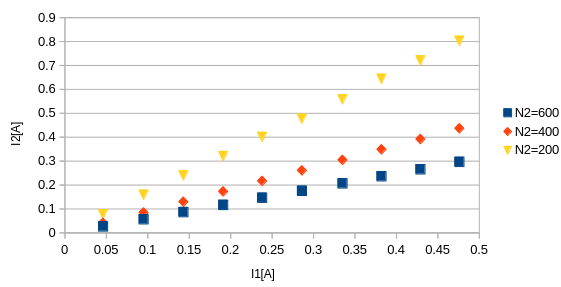
\includegraphics[scale=0.8]{images/2.png}
\end{center}

% subsection zaleznosc (end)

\pagebreak
\subsection{Sprawnosc Transformatora}\label{sub:sprawnosc_transformatora} % (fold)
\begin{center}
	\large Zależność napięcia od natężenia prądu w obwodzie wtórnym
	$U_2 = f(I_2)$
	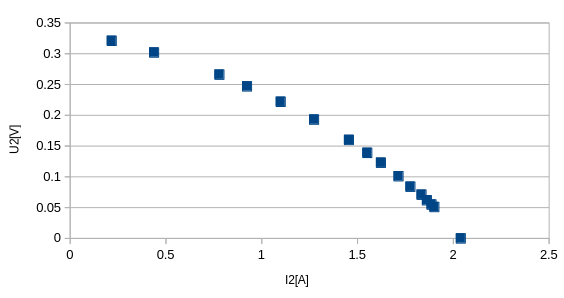
\includegraphics[scale=0.8]{images/3.png}
\end{center}
\subsubsection{Obliczenia}

Sprawność transformatora obliczona na podstawie wzoru:
\[
	\eta = \frac{U_2I_2}{U_1I_1} \cdot 100\%
\]

Dla $R = 0$ jest to:
\[
	\eta_0 = \frac{0,217 \cdot 0,321}{4,28 \cdot 0,174} \cdot 100\% = 9,35\%
\]

\begin{center}
	\begin{tabular}{|l|l|l|l|l|l|}
		\hline
		R        & $U_1$ & $I_1$ & $U_2$ & $I_2$ & sprawność  \\ \hline
		0        & 4.28  & 0.174 & 0.217 & 0.321 & 9.3534482 \\ \hline
		1        & 4.28  & 0.164 & 0.438 & 0.302 & 18.844882 \\ \hline
		2        & 4.28  & 0.145 & 0.779 & 0.266 & 33.389300 \\ \hline
		3        & 4.28  & 0.136 & 0.923 & 0.247 & 39.166609 \\ \hline
		4        & 4.28  & 0.122 & 1.099 & 0.222 & 46.724758 \\ \hline
		6        & 4.28  & 0.108 & 1.273 & 0.193 & 53.151825 \\ \hline
		8        & 4.28  & 0.09  & 1.455 & 0.16  & 60.436137 \\ \hline
		10       & 4.28  & 0.081 & 1.551 & 0.139 & 62.186742 \\ \hline
		12       & 4.28  & 0.072 & 1.622 & 0.123 & 64.741043 \\ \hline
		16       & 4.28  & 0.061 & 1.714 & 0.101 & 66.306879 \\ \hline
		20       & 4.3   & 0.053 & 1.776 & 0.084 & 65.460289 \\ \hline
		24       & 4.32  & 0.047 & 1.834 & 0.071 & 64.132190 \\ \hline
		28       & 4.32  & 0.043 & 1.862 & 0.062 & 62.146856 \\ \hline
		32       & 4.32  & 0.04  & 1.886 & 0.055 & 60.028935 \\ \hline
		34       & 4.34  & 0.038 & 1.901 & 0.051 & 58.786684 \\ \hline
		$\infty$ & 4.35  & 0.022 & 2.039 & 0     & 0         \\ \hline
	\end{tabular}

	\vspace{1cm}
	\large Zależność sprawności transformatora od natężenia prądu w uzwojeniu wtórnym $\eta = f(I2)$

	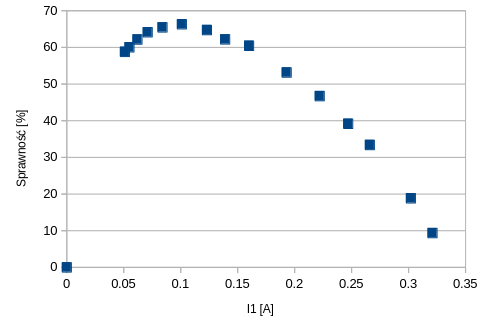
\includegraphics[scale=0.8]{images/sprawnosc.png}
\end{center}


% subsection Sprawnosc Transformatora (end)

\section{Wnioski}\label{sub:wnioski} % (fold)
Różnice pomiędzy wartościami teoretycznymi, a wyliczonymi może wynikać z cech tranzystora oraz zjawisk nieuwzględnionych podczas obliczeń.
% subsection Wnioski (end)


\end{document}

